\documentclass[12pt,a4paper]{article}

\usepackage[utf8]{inputenc}
\usepackage[T1]{fontenc}
\usepackage{lmodern}
\usepackage{graphicx}
\usepackage{amsmath,amssymb}
\usepackage{geometry}
\usepackage{hyperref}
\usepackage{xcolor}
\usepackage{listings}
\usepackage{microtype}
\usepackage{float}
\usepackage{booktabs}
\usepackage{tabularx}
\usepackage{tikz}

\graphicspath{{./}{./screenshots/}}
\DeclareGraphicsExtensions{.pdf,.png,.jpg,.jpeg,.PNG,.JPG,.JPEG}
\usetikzlibrary{shapes.geometric, arrows.meta, positioning, calc, fit, backgrounds, shadows, decorations.pathreplacing}

\geometry{margin=1in}

% Configure completely empty page style (no page numbers on any page)
\pagestyle{empty}
\makeatletter
\let\ps@plain\ps@empty
\makeatother

% Set figure caption prefix to "Fig" as requested
\renewcommand{\figurename}{Fig}

% Section and float numbering formatted as 2.x without Chapter header
\renewcommand{\thesection}{2.\arabic{section}}
\renewcommand{\thefigure}{2.\arabic{figure}}
\renewcommand{\thetable}{2.\arabic{table}}
\AtBeginDocument{\renewcommand{\thelstlisting}{2.\arabic{lstlisting}}}

% Colors for Listings and Hyperlinks
\definecolor{codegreen}{rgb}{0.13,0.55,0.13}
\definecolor{codegray}{rgb}{0.45,0.45,0.45}
\definecolor{codepurple}{rgb}{0.58,0,0.82}
\definecolor{backcolour}{rgb}{0.97,0.98,0.99}
\definecolor{navyblue}{rgb}{0.0,0.2,0.5}
\definecolor{darkcyan}{rgb}{0.0,0.45,0.45}
\definecolor{bordergray}{rgb}{0.8,0.8,0.8}

\hypersetup{
    colorlinks=true,
    linkcolor=navyblue,
    filecolor=magenta,      
    urlcolor=darkcyan,
    citecolor=navyblue
}

% C++ Listings Setup
\lstdefinestyle{cppstyle}{
    backgroundcolor=\color{backcolour},   
    commentstyle=\color{codegreen}\itshape,
    keywordstyle=\color{navyblue}\bfseries,
    numberstyle=\tiny\color{codegray},
    stringstyle=\color{codepurple},
    basicstyle=\ttfamily\footnotesize,
    breakatwhitespace=false,         
    breaklines=true,                 
    captionpos=b,                    
    keepspaces=true,                 
    numbers=left,                    
    numbersep=7pt,                  
    showspaces=false,                
    showstringspaces=false,
    showtabs=false,                  
    tabsize=2,
    frame=lines,
    rulecolor=\color{bordergray}
}

% Mermaid / Plain Text Listings Setup
\lstdefinestyle{mermaidstyle}{
    backgroundcolor=\color{backcolour},   
    commentstyle=\color{codegray}\itshape,
    keywordstyle=\color{darkcyan}\bfseries,
    basicstyle=\ttfamily\scriptsize,
    breaklines=true,                 
    captionpos=b,                    
    keepspaces=true,                 
    numbers=none,
    frame=single,
    rulecolor=\color{bordergray}
}

\lstset{style=cppstyle}

\begin{document}

% =====================================================================
% Header: Project Title, Authors, Guide, Department, Institute, Course
% =====================================================================
\noindent
{\Huge \textbf{Hostel Management System}}

\vspace{0.35cm}
\begin{flushright}
\textit{P Sri Eswar Kalyan Raja Reddy (251140)}\\
\textit{M Kesava Ashutosh (251136)}
\end{flushright}

\vspace{0.8cm}

\begin{center}
\begin{tabular}{r@{\quad}l}
\textbf{Guide:} & Dr. Anoop Jacob Thomas \\
\textbf{Department:} & Computer Science and Engineering \\
\textbf{Institute:} & Indian Institute of Information Technology, Tiruchirappalli \\
\textbf{Course stage:} & Second Year, Semester III (C++ OOP Mini-Project)
\end{tabular}
\end{center}

\vspace{1.0cm}

% =====================================================================
% 1.1 Introduction and Problem Statement
% =====================================================================
\section{Introduction and Problem Statement}
\label{sec:intro}
Campus accommodation administration is a critical logistical responsibility within higher educational institutions. It requires managing hundreds or thousands of resident student profiles, maintaining an accurate inventory of physical rooms across blocks and floors, monitoring dynamic bed capacities, processing room allotments, and swiftly addressing facility maintenance complaints.

Traditionally, university and collegiate hostels have relied heavily on physical paper registers or isolated desktop spreadsheets. These legacy operational methods lead to severe operational challenges:
\begin{itemize}
    \item \textbf{Data Inconsistency and Duplication:} Disparate paper ledgers frequently result in conflicting records of student occupancies, double allocations, and inaccurate vacancy calculations.
    \item \textbf{Administrative Delays:} Room allotment and checkout procedures demand labor-intensive manual lookups, causing long queues during peak academic admission cycles.
    \item \textbf{Grievance Resolution Bottlenecks:} Students submitting paper-based complaints have no transparent mechanism to monitor maintenance progress, resulting in repeated in-person visits to warden offices.
    \item \textbf{Lack of Real-Time Analytics:} Hostel authorities lack instantaneous visibility into aggregate facility metrics, such as overall occupancy rates, vacant bed capacity, and pending maintenance backlogs.
\end{itemize}

To solve these persistent administrative problems, \textbf{HostelOS} was conceived and developed as a modern, full-stack, web-based Hostel Management System grounded in rigorous Object-Oriented Programming (OOPS) principles. 

HostelOS provides decoupled, role-tailored digital portals: a self-service resident student portal and a high-efficiency warden command center. The entire system is anchored by a high-performance C++17 RESTful application server utilizing \texttt{cpp-httplib} and \texttt{nlohmann/json}, integrated with an ACID-compliant MySQL 8.0 relational database engine via the native MySQL C Client API (detailed in Section~\ref{sec:tech_stack}). The user interface leverages lightweight, standards-compliant HTML5, custom CSS design tokens, and vanilla asynchronous JavaScript (Fetch API) without external heavyweight framework overhead.

% =====================================================================
% 6. Scope
% =====================================================================
\section{Scope}
\label{sec:scope}
The scope of the HostelOS project defines the operational and architectural boundaries within which the software functions:

\begin{itemize}
    \item \textbf{User Demarcation and Authentication:} Provision of secure, role-differentiated access controlling two distinct personas:
    \begin{enumerate}
        \item \textit{Resident Students:} Authenticated via numerical university Student ID or institutional email address with individual password protection.
        \item \textit{Hostel Administrators / Wardens:} Authenticated through privileged administrator accounts with administrative oversight.
    \end{enumerate}
    \item \textbf{Student Lifecycle Management:} Managing student profile information (name, institutional email, department, contact number) alongside automated sequential Student ID calculation and collision prevention.
    \item \textbf{Room Inventory and Capacity Tracking:} Tracking physical residential assets categorized by hostel block, floor level, room identifier, total bed capacity, and real-time active occupancy.
    \item \textbf{Transactional Room Allocation:} Automated allotment logic that enforces strict constraint validation: verifying student enrollment, precluding simultaneous multiple active room allotments, and rejecting assignments to rooms operating at maximum capacity.
    \item \textbf{Checkout and Deallocation Workflow:} Systematic recording of resident checkout through timestamped allocation termination, instantly updating room vacancies.
    \item \textbf{Maintenance Grievance Lifecycle:} End-to-end maintenance ticketing enabling residents to register categorized complaints (electrical, plumbing, sanitation, civil repairs) and empowering wardens to transition grievance states through a validated lifecycle (\textit{Pending} $\rightarrow$ \textit{In Progress} $\rightarrow$ \textit{Resolved}).
    \item \textbf{System Demarcation (Out of Current Scope):} Automatic biometric attendance hardware integration, campus-wide gate pass management, and online payment gateway merchant settlements are reserved for future architectural iterations.
\end{itemize}

% =====================================================================
% 7. Feature Set
% =====================================================================
\section{Feature Set}
\label{sec:features}
HostelOS implements a comprehensive suite of features engineered for performance, security, and usability:

\begin{itemize}
    \item \textbf{Feature 1: Dual-Mode Secure Authentication.}
    Residents can authenticate using either their unique numerical Student ID (e.g., \texttt{101}) or registered university email address (e.g., \texttt{karthik.student@example.com}). The login controller automatically determines the credential type and routes verification queries efficiently, while administrator logins are verified against dedicated administrative credential tables.
    
    \item \textbf{Feature 2: Student Directory and Automated Registration.}
    Hostel administrators can onboard new residents seamlessly. The system includes an automated next-available Student ID calculation engine (\texttt{/api/students/next-id}) to eliminate primary key collisions. All inputs undergo length validation and SQL injection sanitization before database insertion.
    
    \item \textbf{Feature 3: Resident Student Portal (Fig~\ref{fig:student_ui}).}
    Authenticated residents access an intuitive, responsive personal dashboard presenting live room details (block designation, floor level, room number), assigned roommates, institutional profile details, and a dedicated ticket submission module.
    
    \item \textbf{Feature 4: Real-Time Room Matrix and Vacancy Inspection.}
    A dynamic room inventory matrix delivers instantaneous status visibility across all blocks. The engine computes live occupancy by executing relational SQL subqueries against active allocations, labeling rooms as \textit{Available}, \textit{Partially Occupied}, or \textit{Full}.
    
    \item \textbf{Feature 5: Capacity-Constrained Room Allocation.}
    Prevents human error during room allotment. The allocation engine programmatically enforces three critical invariants before persisting an allotment:
    \begin{enumerate}
        \item The student must exist in the verified resident registry.
        \item The student must not possess an existing active allocation (\texttt{end\_date IS NULL}).
        \item The selected room's current active occupants must be strictly less than its configured capacity.
    \end{enumerate}

    \item \textbf{Feature 6: Grievance Lodging and Status Triage Workflow.}
    Students lodge detailed maintenance tickets categorized by fault type. Wardens inspect a centralized triage queue and advance ticket progression dynamically (\textit{Pending} $\rightarrow$ \textit{In Progress} $\rightarrow$ \textit{Resolved}), updating live status badges across student interfaces.

    \item \textbf{Feature 7: Warden Analytical KPI Dashboard (Fig~\ref{fig:admin_ui}).}
    An executive control center featuring real-time statistical KPI cards summarizing Total Registered Students, Total Physical Rooms, Current Hostel Occupancy Percentage, Remaining Vacant Beds, and Unresolved Grievances.

    \item \textbf{Feature 8: Framework-Free Modern Design System.}
    A clean, high-performance web interface styled with custom CSS tokens (\texttt{tokens.css}, \texttt{style.css}, \texttt{student.css}), featuring dark mode aesthetics, glassmorphism cards, responsive flex/grid viewports, and toast notifications without third-party JavaScript dependencies.
\end{itemize}

% =====================================================================
% 8. Code Snippets that Demonstrate OOPS Concepts
% =====================================================================
\section{Code Snippets Demonstrating OOP Concepts}
\label{sec:code}
HostelOS is designed around strict Object-Oriented Programming (OOP) paradigms. Rather than relying on unstructured procedural code or monolithic scripts, the backend decomposes domain logic, HTTP routing, serialization, and database interactions into dedicated classes with well-defined boundaries.

\subsection{Encapsulation and Data Hiding}
\label{sec:encapsulation}
Encapsulation is achieved by isolating internal database connection pointers, SQL query construction, and raw query result structures within private member variables of domain classes and API controller classes. External consumers (such as HTTP route dispatchers) can only interact with these objects through public member methods, ensuring that internal database connection handles (\texttt{MYSQL* conn}) cannot be corrupted or manipulated improperly.

\subsection{Domain Modeling and Entity Abstraction}
\label{sec:abstraction}
The \texttt{Student} class encapsulates all resident data attributes and operational methods, abstracting raw database tables into high-level business entities. Listing~\ref{lst:student_cpp} shows the implementation of the \texttt{Student} domain entity from \texttt{Backend/student.cpp}.

\begin{lstlisting}[language=C++, caption={Domain Entity Modeling and Sanitized Insertion (\texttt{Backend/student.cpp})}, label={lst:student_cpp}]
#include <iostream>
#include <mysql.h>

using namespace std;

class Student
{
public:
    int student_id;
    string name;
    string email;
    string department;
    string phone;
    string password;

    // Default constructor initializing default credentials
    Student() : student_id(0), password("student123") {}

    // Parameterized constructor for object instantiation
    Student(int id, string n, string e, string d, string p, string pwd = "student123")
        : student_id(id), name(n), email(e), department(d), phone(p), password(pwd) {}

    // Static persistence method isolating SQL generation & sanitization
    static bool createStudent(MYSQL* conn, int id, const string& name, 
                              const string& email, const string& department, 
                              const string& phone, const string& password, 
                              string& errMsg)
    {
        if (conn == NULL) {
            errMsg = "Database connection not initialized";
            return false;
        }

        char escName[205], escEmail[205], escDept[105], escPhone[35], escPwd[515];

        mysql_real_escape_string(conn, escName, name.c_str(), min((int)name.length(), 100));
        mysql_real_escape_string(conn, escEmail, email.c_str(), min((int)email.length(), 100));
        mysql_real_escape_string(conn, escDept, department.c_str(), min((int)department.length(), 50));
        mysql_real_escape_string(conn, escPhone, phone.c_str(), min((int)phone.length(), 15));
        mysql_real_escape_string(conn, escPwd, password.c_str(), min((int)password.length(), 255));

        string query = "INSERT INTO students (student_id, name, email, department, phone, password) VALUES (" +
                       to_string(id) + ", '" +
                       string(escName) + "', '" +
                       string(escEmail) + "', '" +
                       string(escDept) + "', '" +
                       string(escPhone) + "', '" +
                       string(escPwd) + "')";

        if (mysql_query(conn, query.c_str()) != 0) {
            errMsg = mysql_error(conn);
            return false;
        }
        return true;
    }
};
\end{lstlisting}

\subsection{Dependency Injection and Resource Management}
\label{sec:dep_injection}
Instead of allowing controllers to instantiate their own database connections—which would lead to resource leaks and tight coupling—HostelOS employs \textbf{Constructor-Based Dependency Injection}. An active, initialized \texttt{MYSQL*} pointer is created once in the \texttt{main()} entry point and injected into each controller instance (\texttt{LoginAPI}, \texttt{StudentAPI}, \texttt{RoomAPI}, \texttt{AllocationAPI}, \texttt{ComplaintAPI}, \texttt{DashboardAPI}).

\subsection{Business Rule Validation and Separation of Concerns}
\label{sec:sep_concerns}
Listing~\ref{lst:allocation_api} illustrates the \texttt{AllocationAPI} controller class from \texttt{Backend/main.cpp}. It encapsulates business validation (student existence, duplicate allocation prevention, room capacity verification) within a dedicated class, cleanly separated from transport routing.

\begin{lstlisting}[language=C++, caption={Controller Encapsulation and Business Rule Validation in \texttt{AllocationAPI}}, label={lst:allocation_api}]
class AllocationAPI {
private:
    MYSQL* conn; // Encapsulated database resource handle
public:
    // Dependency Injection via parameterized constructor
    AllocationAPI(MYSQL* c) : conn(c) {}

    void handleCreateAllocation(const httplib::Request& req, httplib::Response& res) {
        try {
            json data = json::parse(req.body);
            int studentId = data.at("student_id").get<int>();
            int roomId = data.at("room_id").get<int>();

            // 1. Verify that the student exists in the registry
            string checkStudent = "SELECT student_id FROM students WHERE student_id = " 
                                  + to_string(studentId);
            if (mysql_query(conn, checkStudent.c_str()) == 0) {
                MYSQL_RES* resStudent = mysql_store_result(conn);
                if (resStudent && mysql_num_rows(resStudent) == 0) {
                    mysql_free_result(resStudent);
                    res.status = 404;
                    res.set_content(R"({"success":false,"message":"Student does not exist"})", "application/json");
                    return;
                }
                if (resStudent) mysql_free_result(resStudent);
            }

            // 2. Prevent double allocation: ensure student has no active room
            string checkActive = "SELECT allocation_id FROM allocations WHERE student_id = " 
                                 + to_string(studentId) + " AND end_date IS NULL";
            if (mysql_query(conn, checkActive.c_str()) == 0) {
                MYSQL_RES* resActive = mysql_store_result(conn);
                if (resActive && mysql_num_rows(resActive) > 0) {
                    mysql_free_result(resActive);
                    res.status = 409;
                    res.set_content(R"({"success":false,"message":"Student is already allocated to an active room"})", "application/json");
                    return;
                }
                if (resActive) mysql_free_result(resActive);
            }

            // 3. Check Room Capacity constraint against current active allocations
            string checkCap = "SELECT capacity, (SELECT COUNT(*) FROM allocations "
                              "WHERE room_id = " + to_string(roomId) + " AND end_date IS NULL) AS current_occ "
                              "FROM rooms WHERE room_id = " + to_string(roomId);
            if (mysql_query(conn, checkCap.c_str()) == 0) {
                MYSQL_RES* resCap = mysql_store_result(conn);
                if (resCap) {
                    MYSQL_ROW row = mysql_fetch_row(resCap);
                    int capacity = stoi(row[0]);
                    int occupants = stoi(row[1]);
                    mysql_free_result(resCap);
                    if (occupants >= capacity) {
                        res.status = 409;
                        res.set_content(R"({"success":false,"message":"Selected room is already at full capacity"})", "application/json");
                        return;
                    }
                }
            }

            // 4. Persist the new allocation
            string query = "INSERT INTO allocations (student_id, room_id, allocation_date) VALUES (" +
                           to_string(studentId) + ", " + to_string(roomId) + ", CURDATE())";
            if (mysql_query(conn, query.c_str()) == 0) {
                res.status = 201;
                res.set_content(R"({"success":true,"message":"Room allocated successfully"})", "application/json");
            } else {
                res.status = 500;
                res.set_content(R"({"success":false,"message":"Failed to record allocation"})", "application/json");
            }
        } catch (const exception& e) {
            res.status = 400;
            res.set_content(R"({"success":false,"message":"Invalid JSON payload format"})", "application/json");
        }
    }
};
\end{lstlisting}

Listing~\ref{lst:login_api} demonstrates the dual-mode credential authentication logic implemented within \texttt{LoginAPI}, showcasing SQL injection protection and clean conditional routing.

\begin{lstlisting}[language=C++, caption={Dual-Role Authentication Handler with SQL Sanitization (\texttt{Backend/main.cpp})}, label={lst:login_api}]
class LoginAPI {
private:
    MYSQL* conn;
public:
    LoginAPI(MYSQL* c) : conn(c) {}

    void handleLogin(const httplib::Request& req, httplib::Response& res) {
        try {
            json data = json::parse(req.body);
            string userId = data.at("userId").get<string>();
            string password = data.at("password").get<string>();

            char* escPwd = new char[password.length() * 2 + 1];
            char* escUser = new char[userId.length() * 2 + 1];
            mysql_real_escape_string(conn, escPwd, password.c_str(), password.length());
            mysql_real_escape_string(conn, escUser, userId.c_str(), userId.length());

            // 1. Check Administrator credentials first
            string adminQ = "SELECT admin_id FROM admins WHERE username = '" + 
                            string(escUser) + "' AND password = '" + string(escPwd) + "'";
            if (mysql_query(conn, adminQ.c_str()) == 0) {
                MYSQL_RES* adminRes = mysql_store_result(conn);
                if (adminRes && mysql_num_rows(adminRes) > 0) {
                    mysql_free_result(adminRes);
                    delete[] escPwd; delete[] escUser;
                    res.set_content(R"({"success":true,"role":"admin"})", "application/json");
                    return;
                }
                if (adminRes) mysql_free_result(adminRes);
            }

            // 2. Fall back to Student authentication (by ID or Email)
            bool isNumeric = !userId.empty() && userId.find_first_not_of("0123456789") == string::npos;
            string studentQ = isNumeric 
                ? "SELECT student_id, name FROM students WHERE student_id = " + string(escUser) + " AND password = '" + string(escPwd) + "'"
                : "SELECT student_id, name FROM students WHERE email = '" + string(escUser) + "' AND password = '" + string(escPwd) + "'";

            if (mysql_query(conn, studentQ.c_str()) == 0) {
                MYSQL_RES* studentRes = mysql_store_result(conn);
                if (studentRes && mysql_num_rows(studentRes) > 0) {
                    MYSQL_ROW row = mysql_fetch_row(studentRes);
                    json out = {{"success", true}, {"role", "student"}, {"student_id", stoi(row[0])}, {"name", row[1]}};
                    mysql_free_result(studentRes);
                    delete[] escPwd; delete[] escUser;
                    res.set_content(out.dump(), "application/json");
                    return;
                }
                if (studentRes) mysql_free_result(studentRes);
            }
            delete[] escPwd; delete[] escUser;
            res.status = 401;
            res.set_content(R"({"success":false,"message":"Invalid credentials"})", "application/json");
        } catch (...) {
            res.status = 400;
            res.set_content(R"({"success":false,"message":"Malformed login request"})", "application/json");
        }
    }
};
\end{lstlisting}

% =====================================================================
% 9. Architecture Diagram
% =====================================================================
\section{Architecture Diagram}
\label{sec:arch}

\subsection{Multi-Tier Architectural Design}
\label{sec:arch_overview}
HostelOS follows a decoupled three-tier software architecture (with underlying technology stack specifications detailed in Section~\ref{sec:tech_stack}):
\begin{enumerate}
    \item \textbf{Client Presentation Tier (Browser):} Built with semantic HTML5, modern design tokens (\texttt{tokens.css}), and responsive styles. It dispatches asynchronous JSON requests via the standard JavaScript Fetch API to the backend.
    \item \textbf{Application Logic Tier (C++ REST API Server):} An embedded HTTP server listening on port \texttt{8080} that encapsulates request routing, CORS headers, JSON serialization/deserialization, business validation, and OOP controller handlers.
    \item \textbf{Data Persistence Tier (MySQL):} A relational database (\texttt{hostel\_management}) hosting normalized tables for students, rooms, allocations, complaints, and administrators.
\end{enumerate}

\subsection{Multi-Tier Architecture Diagram in TikZ}
\label{sec:arch_tikz}
Figure~\ref{fig:architecture} presents the multi-tier architectural diagram of HostelOS.

\begin{figure}[htbp]
\centering
\resizebox{0.96\textwidth}{!}{%
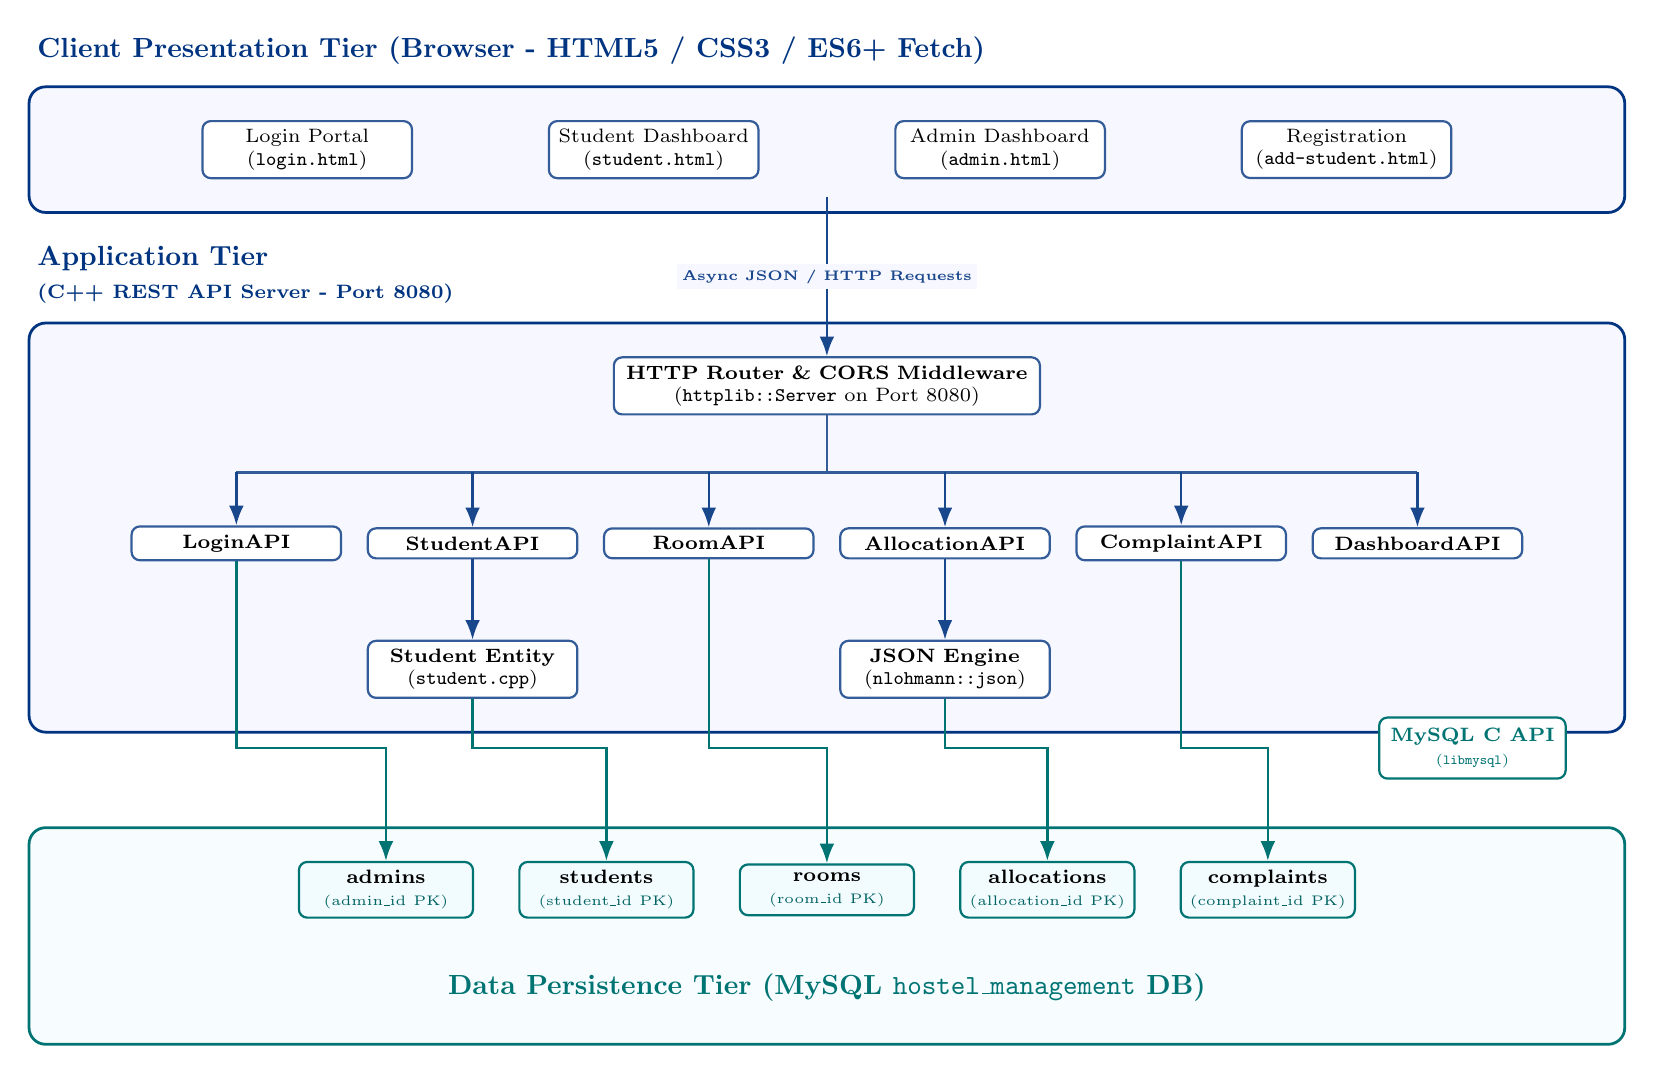
\begin{tikzpicture}[
    font=\sffamily,
    tierbox/.style={draw=navyblue, fill=blue!3, rounded corners=6pt, line width=1pt, inner xsep=18pt, inner ysep=12pt},
    compbox/.style={draw=navyblue!80, fill=white, rounded corners=3pt, line width=0.8pt, align=center, inner sep=3pt, font=\scriptsize, text width=2.45cm},
    apibox/.style={draw=navyblue!80, fill=white, rounded corners=3pt, line width=0.8pt, align=center, inner sep=3pt, font=\scriptsize, text width=2.45cm, minimum width=2.5cm},
    dbbox/.style={draw=darkcyan, fill=cyan!5, rounded corners=3pt, line width=0.8pt, align=center, inner sep=3pt, font=\scriptsize, text width=2.0cm},
    arrow/.style={-{Latex[length=2.5mm]}, line width=0.85pt, color=navyblue!90},
    dbarrow/.style={-{Latex[length=2.5mm]}, line width=0.85pt, color=darkcyan}
]

% ==================== Tier 1: Client Presentation Tier ====================
\coordinate (t1_west) at (-9.5, 0);
\coordinate (t1_east) at (9.5, 0);

\node[compbox] (login_ui)   at (-6.6, 0) {Login Portal\\(\texttt{login.html})};
\node[compbox] (student_ui) at (-2.2, 0) {Student Dashboard\\(\texttt{student.html})};
\node[compbox] (admin_ui)   at (2.2, 0)  {Admin Dashboard\\(\texttt{admin.html})};
\node[compbox] (reg_ui)     at (6.6, 0)  {Registration\\(\texttt{add-student.html})};

\begin{scope}[on background layer]
    \node[tierbox, fit=(login_ui) (reg_ui) (t1_west) (t1_east)] (tier1) {};
\end{scope}
\node[anchor=south west, font=\bfseries\color{navyblue}, yshift=4pt] at (tier1.north west) {Client Presentation Tier (Browser - HTML5 / CSS3 / ES6+ Fetch)};

% ==================== Request Arrow (Tier 1 to Tier 2) ====================
\node[compbox, font=\scriptsize, text width=5.2cm] (router) at (0, -3.0) {\textbf{HTTP Router \& CORS Middleware}\\(\texttt{httplib::Server} on Port 8080)};
\draw[arrow] (0, -0.6) -- (router.north) node[midway, fill=blue!3, inner sep=2pt, font=\tiny\bfseries\color{navyblue}] {Async JSON / HTTP Requests};

% ==================== Tier 2: Backend C++ Application Tier ====================
\coordinate (t2_west) at (-9.5, -5.0);
\coordinate (t2_east) at (9.5, -5.0);

% 6 Controllers with generous width (2.5cm) spaced evenly at x = -7.5, -4.5, -1.5, 1.5, 4.5, 7.5
\node[apibox] (api_login)   at (-7.5, -5.0) {\textbf{LoginAPI}};
\node[apibox] (api_student) at (-4.5, -5.0) {\textbf{StudentAPI}};
\node[apibox] (api_room)    at (-1.5, -5.0) {\textbf{RoomAPI}};
\node[apibox] (api_alloc)   at (1.5, -5.0)  {\textbf{AllocationAPI}};
\node[apibox] (api_comp)    at (4.5, -5.0)  {\textbf{ComplaintAPI}};
\node[apibox] (api_dash)    at (7.5, -5.0)  {\textbf{DashboardAPI}};

% Orthogonal Router Bus
\draw[line width=0.85pt, color=navyblue!80] (router.south) -- (0, -4.1);
\draw[line width=0.85pt, color=navyblue!80] (-7.5, -4.1) -- (7.5, -4.1);
\draw[arrow] (-7.5, -4.1) -- (api_login.north);
\draw[arrow] (-4.5, -4.1) -- (api_student.north);
\draw[arrow] (-1.5, -4.1) -- (api_room.north);
\draw[arrow] (1.5, -4.1)  -- (api_alloc.north);
\draw[arrow] (4.5, -4.1)  -- (api_comp.north);
\draw[arrow] (7.5, -4.1)  -- (api_dash.north);

% Internal Tier 2 Domain Entities
\node[compbox, text width=2.45cm] (entity_student) at (-4.5, -6.6) {\textbf{Student Entity}\\(\texttt{student.cpp})};
\node[compbox, text width=2.45cm] (json_engine)    at (1.5, -6.6)  {\textbf{JSON Engine}\\(\texttt{nlohmann::json})};

\draw[arrow] (api_student.south) -- (entity_student.north);
\draw[arrow] (api_alloc.south)   -- (json_engine.north);

\begin{scope}[on background layer]
    % Generous fit spanning symmetrically to +/- 9.5cm at Tier 2 level
    \node[tierbox, fit=(router) (api_login) (api_dash) (entity_student) (json_engine) (t2_west) (t2_east)] (tier2) {};
\end{scope}
% Wrapped title anchored at top-left
\node[anchor=south west, align=left, font=\bfseries\color{navyblue}, yshift=3pt] at (tier2.north west) {Application Tier\\\scriptsize (C++ REST API Server - Port 8080)};

% ==================== Tier 3: Data Persistence Tier ====================
\coordinate (t3_west) at (-9.5, -9.4);
\coordinate (t3_east) at (9.5, -9.4);

% 5 DB Tables spaced evenly across x = -5.6, -2.8, 0.0, 2.8, 5.6
\node[dbbox] (tb_admin) at (-5.6, -9.4) {\textbf{admins}\\{\tiny\color{darkcyan!85!black}(admin\_id PK)}};
\node[dbbox] (tb_stud)  at (-2.8, -9.4) {\textbf{students}\\{\tiny\color{darkcyan!85!black}(student\_id PK)}};
\node[dbbox] (tb_room)  at (0.0, -9.4)  {\textbf{rooms}\\{\tiny\color{darkcyan!85!black}(room\_id PK)}};
\node[dbbox] (tb_alloc) at (2.8, -9.4)  {\textbf{allocations}\\{\tiny\color{darkcyan!85!black}(allocation\_id PK)}};
\node[dbbox] (tb_comp)  at (5.6, -9.4)  {\textbf{complaints}\\{\tiny\color{darkcyan!85!black}(complaint\_id PK)}};

% Tier 3 Title placed safely at the bottom where no arrows cross
\node[anchor=north, font=\bfseries\color{darkcyan}, yshift=-4pt] (tier3_lbl) at (0, -10.2) {Data Persistence Tier (MySQL \texttt{hostel\_management} DB)};

\begin{scope}[on background layer]
    \node[tierbox, fit=(tb_admin) (tb_comp) (tier3_lbl) (t3_west) (t3_east), draw=darkcyan, fill=cyan!3] (tier3) {};
\end{scope}

% Dedicated API Bridge Label (Safely placed at x = 7.0 to 9.2, with over 1.4cm clear space to line at x = 5.6)
\node[draw=darkcyan, fill=white, rounded corners=3pt, line width=0.8pt, font=\scriptsize\bfseries\color{darkcyan}, align=center, inner sep=4pt, anchor=west] at (7.0, -7.6) {MySQL C API\\{\tiny\mdseries(\texttt{libmysql})}};

% Direct Parallel Database Connectors (Lines end cleanly at x = -5.6, -2.8, 0.0, 2.8, 5.6 with zero overlap)
\draw[dbarrow] (api_login.south)      |- (-5.6, -7.6) -- (tb_admin.north);
\draw[dbarrow] (entity_student.south) |- (-2.8, -7.6) -- (tb_stud.north);
\draw[dbarrow] (api_room.south)       |- (0.0, -7.6)  -- (tb_room.north);
\draw[dbarrow] (json_engine.south)    |- (2.8, -7.6)  -- (tb_alloc.north);
\draw[dbarrow] (api_comp.south)       |- (5.6, -7.6)  -- (tb_comp.north);

\end{tikzpicture}
}
\caption{Multi-Tier System Architecture of HostelOS (Presentation, Application, and Persistence Tiers)}
\label{fig:architecture}
\end{figure}

\subsection{Mermaid Architecture Specification from \texttt{architecture\_diagram.md}}
\label{sec:arch_mermaid}
Listing~\ref{lst:arch_mermaid} contains the verbatim Mermaid architecture code sourced directly from \texttt{architecture\_diagram.md}.

\begin{lstlisting}[style=mermaidstyle, caption={Mermaid Architecture Code from \texttt{architecture\_diagram.md}}, label={lst:arch_mermaid}]
graph TD
    subgraph Client ["Client Presentation Tier (Browser)"]
        UI_Login["Login Portal (login.html)"]
        UI_Student["Student Dashboard (student.html)"]
        UI_Admin["Admin Dashboard (admin.html)"]
        UI_AddStudent["Student Registration (add-student.html)"]
    end

    subgraph Backend ["Application Tier (C++ REST API Server - Port 8080)"]
        Router["HTTP Router & CORS Middleware<br/>(httplib::Server)"]
        
        subgraph OOP_Controllers ["OOP Controllers & Domain Handlers"]
            LoginAPI["LoginAPI"]
            StudentAPI["StudentAPI"]
            ComplaintAPI["ComplaintAPI"]
            DashboardAPI["DashboardAPI"]
            RoomAPI["RoomAPI"]
            AllocationAPI["AllocationAPI"]
        end

        StudentModel["Student Domain Entity<br/>(student.cpp)"]
        JSONParser["JSON Engine<br/>(nlohmann::json)"]
    end

    subgraph DataTier ["Data Persistence Tier (MySQL)"]
        MySQL_Client["MySQL C API (mysql.h / libmysql)"]
        DB[("hostel_management DB")]
        
        T_Students[("students")]
        T_Rooms[("rooms")]
        T_Allocations[("allocations")]
        T_Complaints[("complaints")]
        T_Admins[("admins")]
    end

    Client -->|Async JSON / HTTP Requests| Router
    Router --> OOP_Controllers
    OOP_Controllers <--> JSONParser
    OOP_Controllers --> StudentModel
    OOP_Controllers --> MySQL_Client
    MySQL_Client <--> DB
    DB --- T_Students
    DB --- T_Rooms
    DB --- T_Allocations
    DB --- T_Complaints
    DB --- T_Admins
\end{lstlisting}

% =====================================================================
% Technology Stack
% =====================================================================
\section{Technology Stack}
\label{sec:tech_stack}
HostelOS is engineered as an enterprise-grade, multi-tier hostel management platform that bridges high-performance system programming with modern, lightweight web technologies. Rather than relying on heavyweight, multi-gigabyte frameworks with substantial runtime overhead and complex dependency trees, HostelOS embraces modern standards, single-header C++ libraries, native database drivers, and framework-free client rendering. This section outlines the technologies, tools, and design rationales powering each operational tier of the system.

\subsection{Tier-by-Tier Technology Architecture}
\label{sec:tech_tiers}

\subsubsection{Client Presentation Tier (Frontend)}
The presentation layer provides intuitive, role-tailored dashboards for students and hostel administrators without requiring third-party JavaScript application frameworks:
\begin{itemize}
    \item \textbf{HTML5 (HyperText Markup Language 5):} Employs semantic document structure (\texttt{<header>}, \texttt{<main>}, \texttt{<section>}, \texttt{<article>}, \texttt{<nav>}) across all application views:
    \begin{itemize}
        \item \texttt{login.html}: Unified dual-role authentication portal accepting numerical Student IDs or institutional emails.
        \item \texttt{student.html}: Resident personal dashboard showcasing real-time room allocations, roommate details, and grievance tracking.
        \item \texttt{admin.html}: Warden analytical cockpit featuring live KPI metric cards, room matrix visualization, and grievance triage controls.
        \item \texttt{add-student.html}: Dedicated student registration and onboarding portal featuring automated Student ID calculation.
    \end{itemize}
    \item \textbf{CSS3 with Custom Design Tokens:} Implemented across modular stylesheets (\texttt{tokens.css}, \texttt{style.css}, \texttt{student.css}) using modern design paradigms:
    \begin{itemize}
        \item \textit{CSS Custom Properties (Variables):} Centralized design tokens for curated dark-mode color palettes (deep navy, slate, cyan, and violet accents), spacing scales, and typography hierarchies.
        \item \textit{Glassmorphism and Depth:} Multi-layered translucent card surfaces styled with \texttt{backdrop-filter: blur(12px)} and subtle border gradients.
        \item \textit{Responsive Grid and Flexbox:} Fluid viewport adaptation across mobile, tablet, and desktop display resolutions.
        \item \textit{Dynamic Micro-Interactions:} Smooth CSS transitions for button hover states, modal dialog overlays, and animated status badges (\textit{Pending}, \textit{In Progress}, \textit{Resolved}).
    \end{itemize}
    \item \textbf{Vanilla JavaScript (ECMAScript 2020+):}
    \begin{itemize}
        \item \textit{Asynchronous Fetch API:} Dispatches non-blocking asynchronous HTTP requests (\texttt{GET}, \texttt{POST}, \texttt{PUT}) to the C++ backend using \texttt{async/await} constructs and native Promise pipelines.
        \item \textit{Dynamic DOM Manipulation:} Updates dashboard KPI metrics, table rows, and status badges in real time without triggering full-page browser reloads.
        \item \textit{Zero External Dependencies:} Eliminates heavy dependencies (such as React, Angular, or Vue), ensuring sub-50ms initial page load times and zero NPM supply-chain vulnerabilities.
        \item \textit{Client-Side Session Handling:} Utilizes browser \texttt{sessionStorage} to maintain authenticated student and warden session contexts.
    \end{itemize}
\end{itemize}

\subsubsection{Application Logic Tier (Backend REST Server)}
The core business logic, input sanitization, database interaction, and HTTP routing are encapsulated in a high-performance C++ backend:
\begin{itemize}
    \item \textbf{C++17 (ISO/IEC 14882:2017) \cite{cpp17}:} The primary implementation language, chosen for its deterministic execution speed, minimal runtime memory footprint ($<15\,\text{MB}$ RAM), and comprehensive Object-Oriented Programming (OOP) facilities. Modern C++ features utilized include:
    \begin{itemize}
        \item RAII (Resource Acquisition Is Initialization) for automatic database connection and statement cleanup.
        \item Structured bindings, \texttt{std::string\_view}, and standard containers (\texttt{std::vector}, \texttt{std::map}) for efficient in-memory processing.
        \item Strict encapsulation through modular API controller classes (\texttt{LoginAPI}, \texttt{StudentAPI}, \texttt{RoomAPI}, \texttt{AllocationAPI}, \texttt{ComplaintAPI}, \texttt{DashboardAPI}).
    \end{itemize}
    \item \textbf{cpp-httplib HTTP Server \cite{httplib}:} A lightweight, header-only C++11/17 HTTP/HTTPS server library (\texttt{httplib.h}) authored by Yuji Hirose:
    \begin{itemize}
        \item Provides a multi-threaded worker thread pool handling concurrent client connections over TCP port \texttt{8080}.
        \item Implements RESTful HTTP method routing (\texttt{Get}, \texttt{Post}, \texttt{Put}, \texttt{Options}) with regex path matching for parameterized endpoints (e.g., \texttt{/api/students/:id}, \texttt{/api/complaints/:id}).
        \item Embeds Cross-Origin Resource Sharing (CORS) middleware, enabling decoupled client-server hosting.
    \end{itemize}
    \item \textbf{nlohmann/json Engine \cite{nlohmann}:} Modern JSON parser and serializer for C++ (\texttt{json.hpp}) authored by Niels Lohmann:
    \begin{itemize}
        \item Single-header, intuitive JSON construction allowing direct mapping between relational SQL tuples and RESTful JSON payloads.
        \item Provides type-safe casting, deserialization error trapping, and structured payload extraction.
    \end{itemize}
    \item \textbf{MySQL C Client API (\texttt{mysql.h} / \texttt{libmysql}) \cite{mysql}:}
    \begin{itemize}
        \item Native binary client connector providing direct, low-latency communication with the MySQL database engine.
        \item Implements connection lifecycle management via \texttt{mysql\_init()}, \texttt{mysql\_real\_connect()}, \texttt{mysql\_query()}, and \texttt{mysql\_close()}.
        \item Safeguards against SQL injection attacks by escaping dynamic user inputs through \texttt{mysql\_real\_escape\_string()}.
    \end{itemize}
\end{itemize}

\subsubsection{Data Persistence Tier (Relational Database)}
\begin{itemize}
    \item \textbf{MySQL Database Server 8.0+ / MariaDB 10.4+ \cite{mysql}:} Enterprise-grade open-source relational database management system.
    \item \textbf{InnoDB Storage Engine:} Provides full ACID (Atomicity, Consistency, Isolation, Durability) transactional guarantees, preventing database corruption during concurrent room allocations.
    \item \textbf{Relational Integrity and Constraints:}
    \begin{itemize}
        \item Foreign key constraints with cascading operations ensure referential consistency between students, room allotments, and maintenance complaints.
        \item Unique key indexing on Student Email (\texttt{email}) and Room Designation (\texttt{room\_number}) prevents duplicate onboarding and room duplication.
        \item Normalized to Third Normal Form (3NF) to eliminate transitive dependencies and operational update anomalies.
    \end{itemize}
\end{itemize}

\subsubsection{Development, Compilation, and Toolchain Environment}
\begin{itemize}
    \item \textbf{Compilers:} GCC / MinGW-w64 (v9.0+ / v11.0+) with flags \texttt{-std=c++17 -O2 -lmysql -lws2\_32 -lpthread}; MSVC 2019/2022 supported.
    \item \textbf{Networking \& Threading:} Windows Sockets 2 (\texttt{ws2\_32.lib}) and POSIX Threads (\texttt{pthread}) for worker thread pooling.
    \item \textbf{Configuration:} Database credentials decoupled into environment variables (\texttt{HOSTEL\_DB\_HOST}, \texttt{HOSTEL\_DB\_USER}, \texttt{HOSTEL\_DB\_PASSWORD}, \texttt{HOSTEL\_DB\_NAME}).
    \item \textbf{Documentation \& Modeling:} \LaTeX{} with TikZ for formal report figures; Mermaid.js for design diagrams.
\end{itemize}

\subsection{Technology Stack Summary Matrix}
\label{sec:tech_table}
Table~\ref{tab:tech_stack} summarizes the technologies, libraries, and protocols comprising the HostelOS architecture.

\begin{table}[H]
\centering
\footnotesize
\setlength{\tabcolsep}{5pt}
\renewcommand{\arraystretch}{1.1}
\begin{tabularx}{\textwidth}{p{2.5cm} p{3.6cm} X}
\toprule
\textbf{Layer / Tier} & \textbf{Technology \& Version} & \textbf{Architectural Role \& Capability} \\
\midrule
\textbf{Frontend UI}   & HTML5 (W3C Standard)            & Semantic page structure and form scaffolding across all 4 portals. \\
\textbf{Styling}       & CSS3 (Tokens \& Dark Palette)  & Modern design tokens (\texttt{tokens.css}), glassmorphism, responsive flex/grid. \\
\textbf{Client Logic}  & JavaScript (ES2020+ Fetch API)  & Asynchronous non-blocking REST calls, DOM mutations, and session state. \\
\textbf{Backend Lang.} & C++ (ISO C++17 Standard)        & Domain business logic, controllers, and deterministic memory management via RAII. \\
\textbf{Web Server}    & cpp-httplib (v0.14+ single-hdr) & Multi-threaded embedded HTTP server on port 8080, route dispatching, CORS. \\
\textbf{Serialization} & nlohmann/json (v3.11+)          & High-speed JSON serialization/deserialization and REST payload validation. \\
\textbf{DB Connector}  & MySQL C API (\texttt{mysql.h}) & Low-latency direct socket connection, SQL execution, and injection escaping. \\
\textbf{Database}      & MySQL 8.0+ / MariaDB 10.4+      & 3NF relational persistence, ACID guarantees, foreign keys, InnoDB engine. \\
\textbf{Build Tools}   & MinGW-w64 / MSVC 2019+          & Native binary compilation with flags \texttt{-std=c++17 -O2 -lmysql -lws2\_32}. \\
\textbf{Protocol}      & HTTP/1.1 REST (RFC 7230)        & Stateless async client-server communication using standard HTTP verbs. \\
\bottomrule
\end{tabularx}
\caption{HostelOS Technology Stack and Component Specifications}
\label{tab:tech_stack}
\end{table}

\subsection{Architectural Rationale and Design Justifications}
\label{sec:tech_justification}
The selection of the HostelOS technology stack was driven by core engineering principles:

\begin{enumerate}
    \item \textbf{C++17 Backend vs. Interpreted Runtimes:} C++ provides deterministic memory management, sub-millisecond route response latencies, and zero garbage-collection jitter. The compiled native binary consumes under 15\,MB of RAM, compared to 200--500\,MB typical of Node.js or JVM runtimes.
    
    \item \textbf{Single-Header C++ Libraries (\texttt{cpp-httplib} \& \texttt{nlohmann/json}):} Utilizing single-header libraries eliminates external package manager dependencies, CMake build cascades, and linker discrepancies across Windows (MinGW) and Linux (GCC).
    
    \item \textbf{Vanilla Client-Side Stack vs. Heavy Frameworks:} Avoiding heavy SPA frameworks (React/Angular) removes large \texttt{node\_modules} overhead and compilation pipelines, ensuring instant page loads, zero build steps, and native browser compatibility.
    
    \item \textbf{Relational ACID Database vs. NoSQL:} Hostel room allocation requires strict referential integrity—preventing overbooking and simultaneous active student allocations. MySQL's InnoDB engine enforces atomic transactions, foreign key cascades, and row-level locks.
\end{enumerate}

% =====================================================================
% 10. Database Schema and ER Diagram
% =====================================================================
\section{Database Schema and ER Diagram}
\label{sec:db}

\subsection{Relational Schema Specifications}
\label{sec:db_specs}
The persistence layer of HostelOS is implemented on MySQL Server 8.0 with InnoDB storage engine tables, ensuring ACID compliance, row-level locking, and strict foreign key integrity. The relational design satisfies Third Normal Form (3NF), minimizing data redundancy. Table~\ref{tab:db_schema} outlines the relational schema specifications.

\begin{table}[H]
\centering
\footnotesize
\setlength{\tabcolsep}{5pt}
\renewcommand{\arraystretch}{1.1}
\begin{tabularx}{\textwidth}{p{2.0cm} p{2.2cm} p{3.2cm} X}
\toprule
\textbf{Table Name} & \textbf{Primary Key} & \textbf{Foreign Keys} & \textbf{Attributes \& Constraints} \\
\midrule
\texttt{students}    & \texttt{student\_id}    & None & \texttt{name} VARCHAR(100), \texttt{email} VARCHAR(100) UNIQUE, \texttt{department} VARCHAR(50), \texttt{phone} VARCHAR(15), \texttt{password} VARCHAR(255). \\
\texttt{rooms}       & \texttt{room\_id}       & None & \texttt{room\_number} VARCHAR(10) UNIQUE, \texttt{block} VARCHAR(20), \texttt{floor} INT, \texttt{capacity} INT. \\
\texttt{allocations} & \texttt{allocation\_id} & \texttt{student\_id} $\rightarrow$ \texttt{students}, \texttt{room\_id} $\rightarrow$ \texttt{rooms} & \texttt{allocation\_date} DATE, \texttt{end\_date} DATE (NULL indicates active occupancy). \\
\texttt{complaints}  & \texttt{complaint\_id}  & \texttt{student\_id} $\rightarrow$ \texttt{students} & \texttt{description} VARCHAR(500), \texttt{status} VARCHAR(20) DEFAULT 'Pending', \texttt{created\_at} TIMESTAMP. \\
\texttt{admins}      & \texttt{admin\_id}      & None & \texttt{username} VARCHAR(50) UNIQUE, \texttt{password} VARCHAR(255). \\
\bottomrule
\end{tabularx}
\caption{HostelOS Relational Database Schema Specifications}
\label{tab:db_schema}
\end{table}

\subsection{Database Relational ER Diagram in TikZ}
\label{sec:er_tikz}
Figure~\ref{fig:er_schema} illustrates the relational entity structures, primary keys, and foreign key associations across the database.

\begin{figure}[H]
\centering
\resizebox{0.92\textwidth}{!}{%
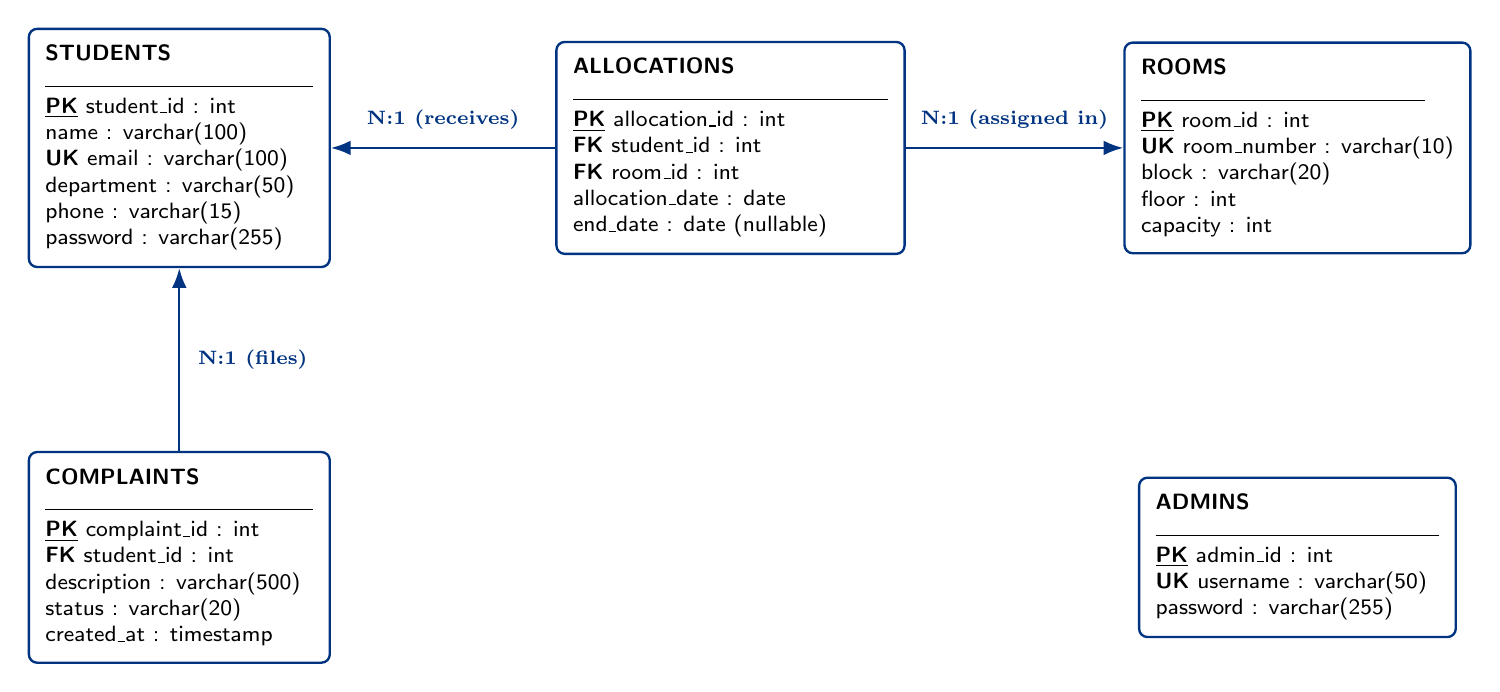
\begin{tikzpicture}[
    font=\sffamily\footnotesize,
    tablebox/.style={draw=navyblue, fill=white, rounded corners=3pt, line width=0.85pt, align=left, inner sep=6pt},
    arrow/.style={-{Latex[length=2.5mm]}, line width=0.85pt, color=navyblue}
]

% Top Row: STUDENTS (left), ALLOCATIONS (center), ROOMS (right) with ample spacing
\node[tablebox] (stud) at (0, 2) {
    \textbf{STUDENTS} \\
    \rule{3.4cm}{0.4pt} \\
    \underline{\textbf{PK}} student\_id : int \\
    name : varchar(100) \\
    \textbf{UK} email : varchar(100) \\
    department : varchar(50) \\
    phone : varchar(15) \\
    password : varchar(255)
};

\node[tablebox] (alloc) at (7.0, 2) {
    \textbf{ALLOCATIONS} \\
    \rule{4.0cm}{0.4pt} \\
    \underline{\textbf{PK}} allocation\_id : int \\
    \textbf{FK} student\_id : int \\
    \textbf{FK} room\_id : int \\
    allocation\_date : date \\
    end\_date : date (nullable)
};

\node[tablebox] (rooms) at (14.2, 2) {
    \textbf{ROOMS} \\
    \rule{3.6cm}{0.4pt} \\
    \underline{\textbf{PK}} room\_id : int \\
    \textbf{UK} room\_number : varchar(10) \\
    block : varchar(20) \\
    floor : int \\
    capacity : int
};

% Bottom Row: COMPLAINTS (left), ADMINS (right)
\node[tablebox] (comp) at (0, -3.2) {
    \textbf{COMPLAINTS} \\
    \rule{3.4cm}{0.4pt} \\
    \underline{\textbf{PK}} complaint\_id : int \\
    \textbf{FK} student\_id : int \\
    description : varchar(500) \\
    status : varchar(20) \\
    created\_at : timestamp
};

\node[tablebox] (admin) at (14.2, -3.2) {
    \textbf{ADMINS} \\
    \rule{3.6cm}{0.4pt} \\
    \underline{\textbf{PK}} admin\_id : int \\
    \textbf{UK} username : varchar(50) \\
    password : varchar(255)
};

% Clean connectors with labels perfectly centered in wide whitespace channels
\draw[arrow] (alloc) -- node[midway, above=3pt, font=\scriptsize\bfseries\color{navyblue}] {N:1 (receives)} (stud);
\draw[arrow] (alloc) -- node[midway, above=3pt, font=\scriptsize\bfseries\color{navyblue}] {N:1 (assigned in)} (rooms);
\draw[arrow] (comp)  -- node[midway, right=3pt, font=\scriptsize\bfseries\color{navyblue}] {N:1 (files)} (stud);

\end{tikzpicture}
}
\caption{Relational Database Entity-Relationship (ER) Schema and Foreign Key Associations}
\label{fig:er_schema}
\end{figure}

\subsection{Mermaid ER Diagram Snippet from \texttt{README.md}}
\label{sec:er_mermaid}
Listing~\ref{lst:er_mermaid} provides the exact Mermaid entity-relationship diagram snippet from \texttt{README.md}.

\begin{lstlisting}[style=mermaidstyle, caption={Mermaid Entity-Relationship (ER) Diagram Snippet from \texttt{README.md}}, label={lst:er_mermaid}]
erDiagram
    STUDENTS ||--o{ ALLOCATIONS : "receives"
    ROOMS ||--o{ ALLOCATIONS : "assigned in"
    STUDENTS ||--o{ COMPLAINTS : "files"
    ADMINS {
        int admin_id PK
        varchar username UK
        varchar password
    }
    STUDENTS {
        int student_id PK
        varchar name
        varchar email UK
        varchar department
        varchar phone
        varchar password
    }
    ROOMS {
        int room_id PK
        varchar room_number UK
        varchar block
        int floor
        int capacity
    }
    ALLOCATIONS {
        int allocation_id PK
        int student_id FK
        int room_id FK
        date allocation_date
        date end_date
    }
    COMPLAINTS {
        int complaint_id PK
        int student_id FK
        varchar description
        varchar status
        timestamp created_at
    }
\end{lstlisting}

\subsection{Data Definition Language (DDL) Table Schema}
\label{sec:ddl}
Listing~\ref{lst:sql_schema} contains the complete MySQL Data Definition Language (DDL) statements from \texttt{Database/database\_schema.sql}.

\begin{lstlisting}[language=SQL, caption={Relational DDL Table Schema Definitions (\texttt{Database/database\_schema.sql})}, label={lst:sql_schema}]
CREATE DATABASE IF NOT EXISTS hostel_management;
USE hostel_management;

CREATE TABLE IF NOT EXISTS admins (
    admin_id INT PRIMARY KEY AUTO_INCREMENT,
    username VARCHAR(50) NOT NULL UNIQUE,
    password VARCHAR(255) NOT NULL
);

CREATE TABLE IF NOT EXISTS students (
    student_id INT PRIMARY KEY,
    name VARCHAR(100) NOT NULL,
    email VARCHAR(100) NOT NULL UNIQUE,
    department VARCHAR(50) NOT NULL,
    phone VARCHAR(15) NOT NULL,
    password VARCHAR(255) NOT NULL DEFAULT 'student123'
);

CREATE TABLE IF NOT EXISTS rooms (
    room_id INT PRIMARY KEY AUTO_INCREMENT,
    room_number VARCHAR(10) NOT NULL UNIQUE,
    block VARCHAR(20) NOT NULL,
    floor INT NOT NULL,
    capacity INT NOT NULL DEFAULT 2
);

CREATE TABLE IF NOT EXISTS allocations (
    allocation_id INT PRIMARY KEY AUTO_INCREMENT,
    student_id INT NOT NULL,
    room_id INT NOT NULL,
    allocation_date DATE NOT NULL,
    end_date DATE NULL,
    FOREIGN KEY (student_id) REFERENCES students(student_id),
    FOREIGN KEY (room_id) REFERENCES rooms(room_id)
);

CREATE TABLE IF NOT EXISTS complaints (
    complaint_id INT PRIMARY KEY AUTO_INCREMENT,
    student_id INT NOT NULL,
    description VARCHAR(500) NOT NULL,
    status VARCHAR(20) NOT NULL DEFAULT 'Pending',
    created_at TIMESTAMP DEFAULT CURRENT_TIMESTAMP,
    FOREIGN KEY (student_id) REFERENCES students(student_id)
);
\end{lstlisting}

% =====================================================================
% 11. UML Diagrams
% =====================================================================
\section{UML Diagrams}
\label{sec:uml}

\subsection{UML Class Diagram}
\label{sec:class_diag}
The object-oriented design is modeled through a comprehensive UML Class Diagram capturing classes, encapsulated attributes, member methods, and inter-class associations.

Figure~\ref{fig:class_diagram} renders the complete UML Class Diagram in native TikZ.

\begin{figure}[H]
\centering
\resizebox{0.98\textwidth}{!}{%
\begin{tikzpicture}[
    font=\sffamily\scriptsize,
    umlclass/.style={
        draw=navyblue, fill=white, line width=0.85pt, rounded corners=2pt, align=left, inner sep=5pt, text width=4.2cm
    },
    umlwide/.style={
        draw=navyblue, fill=white, line width=0.85pt, rounded corners=2pt, align=left, inner sep=5pt, text width=4.8cm
    },
    rel/.style={-{Latex[length=2.5mm]}, line width=0.85pt, color=navyblue},
    dep/.style={-{Latex[length=2.5mm]}, dashed, line width=0.85pt, color=navyblue},
    comp/.style={{Diamond[fill=navyblue, length=2.8mm]}-{Latex[length=2.5mm]}, line width=0.85pt, color=navyblue}
]

% Server Node (Top Center)
\node[umlclass, text width=4.6cm] (server) at (0, 7.8) {
    \textbf{httplib::Server} \\
    \rule{4.6cm}{0.4pt} \\
    + Post(pattern, handler) : void \\
    + Get(pattern, handler) : void \\
    + Put(pattern, handler) : void \\
    + Options(pattern, handler) : void \\
    + listen(host, port) : void
};

% Row 1: Controllers (x = -6.4, 0.0, 6.4)
\node[umlclass] (login_api) at (-6.4, 3.4) {
    \textbf{\guillemotleft controller\guillemotright\ LoginAPI} \\
    \rule{4.2cm}{0.4pt} \\
    - conn : MYSQL* \\
    \rule{4.2cm}{0.4pt} \\
    + LoginAPI(c : MYSQL*) \\
    + handleLogin(req, res) : void
};

\node[umlclass] (student_api) at (0.0, 3.4) {
    \textbf{\guillemotleft controller\guillemotright\ StudentAPI} \\
    \rule{4.2cm}{0.4pt} \\
    - conn : MYSQL* \\
    \rule{4.2cm}{0.4pt} \\
    + StudentAPI(c : MYSQL*) \\
    + handleGetStudentById(..) : void \\
    + handleGetAllStudents(..) : void \\
    + handleGetNextId(..) : void \\
    + handleCreateStudent(..) : void
};

\node[umlclass] (room_api) at (6.4, 3.4) {
    \textbf{\guillemotleft controller\guillemotright\ RoomAPI} \\
    \rule{4.2cm}{0.4pt} \\
    - conn : MYSQL* \\
    \rule{4.2cm}{0.4pt} \\
    + RoomAPI(c : MYSQL*) \\
    + handleGetRooms(req, res) : void
};

% Row 2: Controllers (x = -6.4, 0.0, 6.4) with ample vertical and horizontal space
\node[umlclass] (alloc_api) at (-6.4, -1.8) {
    \textbf{\guillemotleft controller\guillemotright\ AllocationAPI} \\
    \rule{4.2cm}{0.4pt} \\
    - conn : MYSQL* \\
    \rule{4.2cm}{0.4pt} \\
    + AllocationAPI(c : MYSQL*) \\
    + handleGetAllocations(..) : void \\
    + handleCreateAllocation(..) : void \\
    + handleDeallocate(..) : void
};

\node[umlclass] (comp_api) at (0.0, -1.8) {
    \textbf{\guillemotleft controller\guillemotright\ ComplaintAPI} \\
    \rule{4.2cm}{0.4pt} \\
    - conn : MYSQL* \\
    \rule{4.2cm}{0.4pt} \\
    + ComplaintAPI(c : MYSQL*) \\
    + handleCreateComplaint(..) : void \\
    + handleGetStudentComplaints(..) : void \\
    + handleGetAllComplaints(..) : void \\
    + handleUpdateStatus(..) : void
};

\node[umlclass] (dash_api) at (6.4, -1.8) {
    \textbf{\guillemotleft controller\guillemotright\ DashboardAPI} \\
    \rule{4.2cm}{0.4pt} \\
    - conn : MYSQL* \\
    \rule{4.2cm}{0.4pt} \\
    + DashboardAPI(c : MYSQL*) \\
    + handleGetDashboard(req, res) : void
};

% Domain Entity: Student (Dedicated column on the right, well-separated)
\node[umlwide] (student_class) at (12.8, 1.8) {
    \textbf{\guillemotleft entity\guillemotright\ Student} \\
    \rule{4.8cm}{0.4pt} \\
    + student\_id : int \\
    + name, email : string \\
    + department, phone : string \\
    + password : string \\
    \rule{4.8cm}{0.4pt} \\
    + Student() \\
    + Student(id, n, e, d, p, pwd) \\
    + createStudent(conn, ..) : bool \\
    + addStudent(conn) : void \\
    + viewStudent(conn) : void \\
    + updateStudent(conn) : void \\
    + deleteStudent(conn) : void
};

% Connection Infrastructure (Bottom Center)
\node[umlwide] (mysql_conn) at (0.0, -5.8) {
    \textbf{\guillemotleft external C struct\guillemotright\ MySQLConnection} \\
    \rule{4.8cm}{0.4pt} \\
    + conn : MYSQL* \\
    + connector\_fd : my\_socket
};

% Server Dispatch Composition Connectors
\draw[comp] (server.south) -| (login_api.north);
\draw[comp] (server.south) -- (student_api.north);
\draw[comp] (server.south) -| (room_api.north);

\draw[comp] (login_api.south) -- (alloc_api.north);
\draw[comp] (room_api.south)  -- (dash_api.north);

% Dependency: StudentAPI invokes Student::createStudent()
\draw[dep] (student_api.north) -- ++(0, 1.2) -| node[pos=0.35, above=2pt, font=\scriptsize\bfseries] {invokes createStudent()} (student_class.north);

% Database Associations to MySQLConnection
\draw[rel] (alloc_api.south) |- (mysql_conn.west);
\draw[rel] (comp_api.south)  -- (mysql_conn.north);
\draw[rel] (dash_api.south)  |- (mysql_conn.east);
\draw[rel] (student_class.south) |- (mysql_conn.east);

\end{tikzpicture}
}
\caption{UML Class Diagram specifying Domain Entity, Controller Classes, and System Associations}
\label{fig:class_diagram}
\end{figure}

Listing~\ref{lst:class_mermaid} reproduces the verbatim Mermaid class diagram from \texttt{class\_diagram.md}.

\begin{lstlisting}[style=mermaidstyle, caption={Mermaid UML Class Code from \texttt{class\_diagram.md}}, label={lst:class_mermaid}]
classDiagram
    direction TB

    %% External Infrastructure Types
    class MySQLConnection {
        <<external C struct>>
        MYSQL*
    }

    class HttpServer {
        <<external : httplib::Server>>
        +Post(string pattern, Handler handler)
        +Get(string pattern, Handler handler)
        +Put(string pattern, Handler handler)
        +Options(string pattern, Handler handler)
        +listen(string host, int port)
    }

    %% Domain Entity Class (student.cpp)
    class Student {
        +int student_id
        +string name, email, department, phone, password
        +Student()
        +Student(int id, string n, string e, string d, string p, string pwd)
        +createStudent(conn, id, name, ..)$ bool
        +addStudent(conn) void
        +viewStudent(conn) void
        +updateStudent(conn) void
        +deleteStudent(conn) void
    }

    %% API Controller Classes (main.cpp)
    class LoginAPI {
        -MYSQL* conn
        +LoginAPI(MYSQL* c)
        +handleLogin(Request req, Response res) void
    }

    class StudentAPI {
        -MYSQL* conn
        +StudentAPI(MYSQL* c)
        +handleGetStudentById(..) void
        +handleGetAllStudents(..) void
        +handleGetNextId(..) void
        +handleCreateStudent(..) void
    }

    class ComplaintAPI {
        -MYSQL* conn
        +ComplaintAPI(MYSQL* c)
        +handleCreateComplaint(..) void
        +handleGetStudentComplaints(..) void
        +handleGetAllComplaints(..) void
        +handleUpdateComplaintStatus(..) void
    }

    class DashboardAPI {
        -MYSQL* conn
        +DashboardAPI(MYSQL* c)
        +handleGetDashboard(Request req, Response res) void
    }

    class RoomAPI {
        -MYSQL* conn
        +RoomAPI(MYSQL* c)
        +handleGetRooms(Request req, Response res) void
    }

    class AllocationAPI {
        -MYSQL* conn
        +AllocationAPI(MYSQL* c)
        +handleGetAllocations(..) void
        +handleDeallocate(..) void
        +handleCreateAllocation(..) void
    }

    %% Relationships & Bindings
    StudentAPI ..> Student : invokes createStudent()
    LoginAPI --> MySQLConnection : query
    StudentAPI --> MySQLConnection : query
    ComplaintAPI --> MySQLConnection : query
    DashboardAPI --> MySQLConnection : query
    RoomAPI --> MySQLConnection : query
    AllocationAPI --> MySQLConnection : query
    Student --> MySQLConnection : query

    HttpServer *-- LoginAPI : /api/login
    HttpServer *-- StudentAPI : /api/students
    HttpServer *-- RoomAPI : /api/rooms
    HttpServer *-- AllocationAPI : /api/allocations
    HttpServer *-- ComplaintAPI : /api/complaints
    HttpServer *-- DashboardAPI : /api/admin/dashboard
\end{lstlisting}

\subsection{UML Use Case Diagram}
\label{sec:usecase}
Figure~\ref{fig:use_case} models interactions for the \textbf{Student} and \textbf{Warden / Administrator} actors.

\begin{figure}[H]
\centering
\resizebox{0.95\textwidth}{!}{%
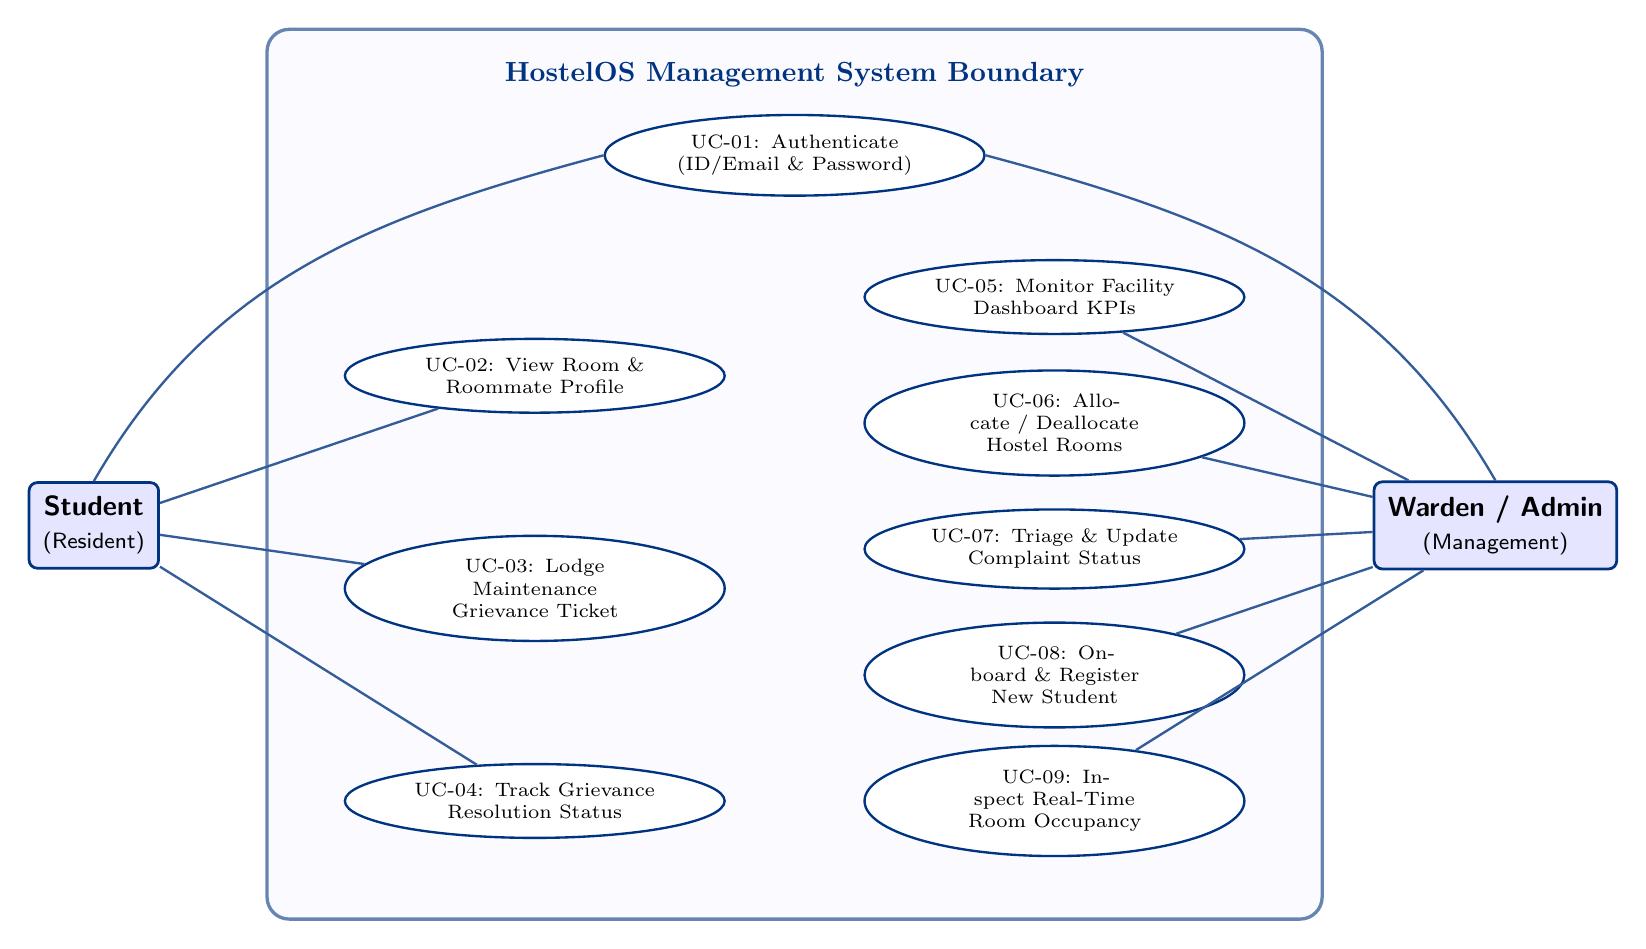
\begin{tikzpicture}[
    font=\sffamily,
    actor/.style={draw=navyblue, line width=1pt, fill=blue!10, rounded corners=3pt, align=center, inner sep=5pt},
    usecase/.style={draw=navyblue, fill=white, ellipse, line width=0.85pt, align=center, inner sep=3pt, font=\scriptsize, text width=3.2cm},
    systembox/.style={draw=navyblue!60, fill=blue!2, rounded corners=8pt, line width=1.2pt},
    assoc/.style={line width=0.85pt, color=navyblue!80}
]

% System Boundary (Spacious and balanced)
\draw[systembox] (0, 0.5) rectangle (13.4, 11.8);
\node[font=\bfseries\color{navyblue}, anchor=north] at (6.7, 11.5) {HostelOS Management System Boundary};

% Actors
\node[actor] (student) at (-2.2, 5.5) {\textbf{Student}\\\footnotesize (Resident)};
\node[actor] (admin)   at (15.6, 5.5) {\textbf{Warden / Admin}\\\footnotesize (Management)};

% Shared Authentication Use Case (Top Center - No Crossing Lines)
\node[usecase] (uc_login) at (6.7, 10.2) {UC-01: Authenticate\\(ID/Email \& Password)};

% Resident Use Cases (Left Column: x = 3.4)
\node[usecase] (uc_profile) at (3.4, 7.4) {UC-02: View Room \&\\Roommate Profile};
\node[usecase] (uc_lodge)   at (3.4, 4.7) {UC-03: Lodge Maintenance\\Grievance Ticket};
\node[usecase] (uc_track)   at (3.4, 2.0) {UC-04: Track Grievance\\Resolution Status};

% Administrative Use Cases (Right Column: x = 10.0)
\node[usecase] (uc_dash)     at (10.0, 8.4) {UC-05: Monitor Facility\\Dashboard KPIs};
\node[usecase] (uc_alloc)    at (10.0, 6.8) {UC-06: Allocate / Deallocate\\Hostel Rooms};
\node[usecase] (uc_triage)   at (10.0, 5.2) {UC-07: Triage \& Update\\Complaint Status};
\node[usecase] (uc_register) at (10.0, 3.6) {UC-08: Onboard \& Register\\New Student};
\node[usecase] (uc_rooms)    at (10.0, 2.0) {UC-09: Inspect Real-Time\\Room Occupancy};

% Associations: Student (Direct, zero crossings)
\draw[assoc] (student.north) to[out=60, in=195] (uc_login.west);
\draw[assoc] (student) -- (uc_profile);
\draw[assoc] (student) -- (uc_lodge);
\draw[assoc] (student) -- (uc_track);

% Associations: Admin (Direct, smooth top arch to UC-01 passing cleanly above UC-05 and UC-06)
\draw[assoc] (admin.north) to[out=120, in=345] (uc_login.east);
\draw[assoc] (admin) -- (uc_dash);
\draw[assoc] (admin) -- (uc_alloc);
\draw[assoc] (admin) -- (uc_triage);
\draw[assoc] (admin) -- (uc_register);
\draw[assoc] (admin) -- (uc_rooms);

\end{tikzpicture}
}
\caption{UML Use Case Diagram for HostelOS depicting Student and Warden operations}
\label{fig:use_case}
\end{figure}

\subsection{UML Activity Diagram}
\label{sec:actdiag}
Figure~\ref{fig:activity_diagram} captures the end-to-end lifecycle of a student maintenance grievance ticket.

\begin{figure}[H]
\centering
\resizebox{0.92\textwidth}{!}{%
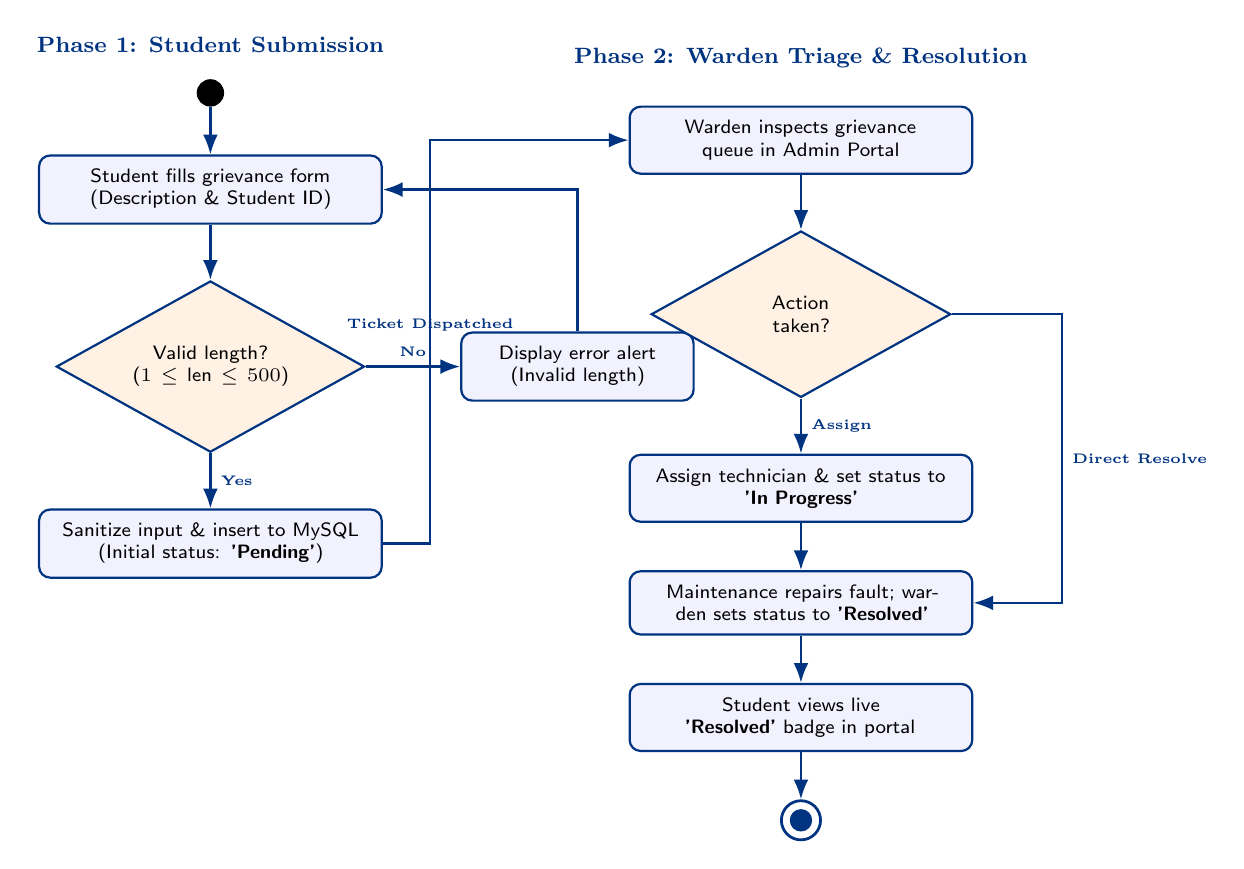
\begin{tikzpicture}[
    font=\sffamily\scriptsize,
    startstop/.style={circle, fill=black, inner sep=3.5pt},
    endstop/.style={circle, draw=navyblue, line width=1pt, fill=navyblue, inner sep=2.5pt},
    outerend/.style={circle, draw=navyblue, line width=1pt, inner sep=5pt},
    activity/.style={draw=navyblue, fill=blue!5, rounded corners=4pt, line width=0.8pt, align=center, inner sep=5pt, text width=4.0cm},
    decision/.style={draw=navyblue, fill=orange!10, diamond, aspect=1.8, line width=0.8pt, align=center, inner sep=3pt, text width=2.4cm},
    arrow/.style={-{Latex[length=2.5mm]}, line width=0.85pt, color=navyblue},
    phasebox/.style={draw=navyblue!40, fill=blue!2, rounded corners=6pt, line width=0.8pt, dashed}
]

% Phase 1: Resident Student Grievance Submission (Left Column: x = 0)
\node[startstop] (start) at (0, 0) {};
\node[activity, below=0.6cm of start] (submit) {Student fills grievance form\\(Description \& Student ID)};
\node[decision, below=0.7cm of submit] (validate) {Valid length?\\($1 \le \text{len} \le 500$)};
\node[activity, right=1.2cm of validate, text width=2.6cm] (error) {Display error alert\\(Invalid length)};
\node[activity, below=0.7cm of validate] (insert) {Sanitize input \& insert to MySQL\\(Initial status: \textbf{'Pending'})};

% Phase 2: Administrative Triage & Resolution (Right Column: x = 7.5)
\node[activity, at={(7.5, -0.6)}] (warden_view) {Warden inspects grievance queue in Admin Portal};
\node[decision, below=0.7cm of warden_view] (triage) {Action\\taken?};
\node[activity, below=0.7cm of triage] (progress) {Assign technician \& set status to\\\textbf{'In Progress'}};
\node[activity, below=0.6cm of progress] (resolve) {Maintenance repairs fault; warden sets status to \textbf{'Resolved'}};
\node[activity, below=0.6cm of resolve] (notify) {Student views live\\\textbf{'Resolved'} badge in portal};
\node[outerend, below=0.6cm of notify] (endout) {};
\node[endstop] at (endout) {};

% Connections - Phase 1
\draw[arrow] (start) -- (submit);
\draw[arrow] (submit) -- (validate);
\draw[arrow] (validate) -- node[above, font=\tiny\bfseries] {No} (error);
\draw[arrow] (error) |- (submit);
\draw[arrow] (validate) -- node[right, font=\tiny\bfseries] {Yes} (insert);

% Bridge between Phase 1 and Phase 2
\draw[arrow] (insert.east) -| ++(0.6, 0) |- (warden_view.west) node[pos=0.25, above, font=\tiny\bfseries] {Ticket Dispatched};

% Connections - Phase 2
\draw[arrow] (warden_view) -- (triage);
\draw[arrow] (triage) -- node[right, font=\tiny\bfseries] {Assign} (progress);
\draw[arrow] (triage.east) -- ++(1.4, 0) |- node[near start, right, font=\tiny\bfseries] {Direct Resolve} (resolve.east);
\draw[arrow] (progress) -- (resolve);
\draw[arrow] (resolve) -- (notify);
\draw[arrow] (notify) -- (endout);

% Phase Headings
\node[font=\footnotesize\bfseries\color{navyblue}, above=6pt of start] {Phase 1: Student Submission};
\node[font=\footnotesize\bfseries\color{navyblue}, at={(7.5, 0.45)}] {Phase 2: Warden Triage \& Resolution};

\end{tikzpicture}
}
\caption{UML Activity Diagram illustrating Grievance Submission and Resolution Lifecycle}
\label{fig:activity_diagram}
\end{figure}

% =====================================================================
% 12. Screenshots
% =====================================================================
\section{Screenshots}
\label{sec:screenshots}
HostelOS features a modern, accessible user interface adhering to design token specifications (\texttt{tokens.css}) with responsive layouts. The client web portal provides live visual feedback for all student and administrative operations.

\subsection{Student Resident Portal Dashboard}
\label{sec:student_screen}
Figure~\ref{fig:student_ui} presents the Student Resident Portal interface. Upon successful authentication, the resident is greeted with their profile summary, assigned room number, hostel block, floor, and registered contact details. The interface incorporates an interactive grievance lodging module with category selection and a dynamic table displaying previously submitted complaints alongside color-coded real-time status badges (\textit{Pending}, \textit{In Progress}, \textit{Resolved}).

\begin{figure}[H]
\centering
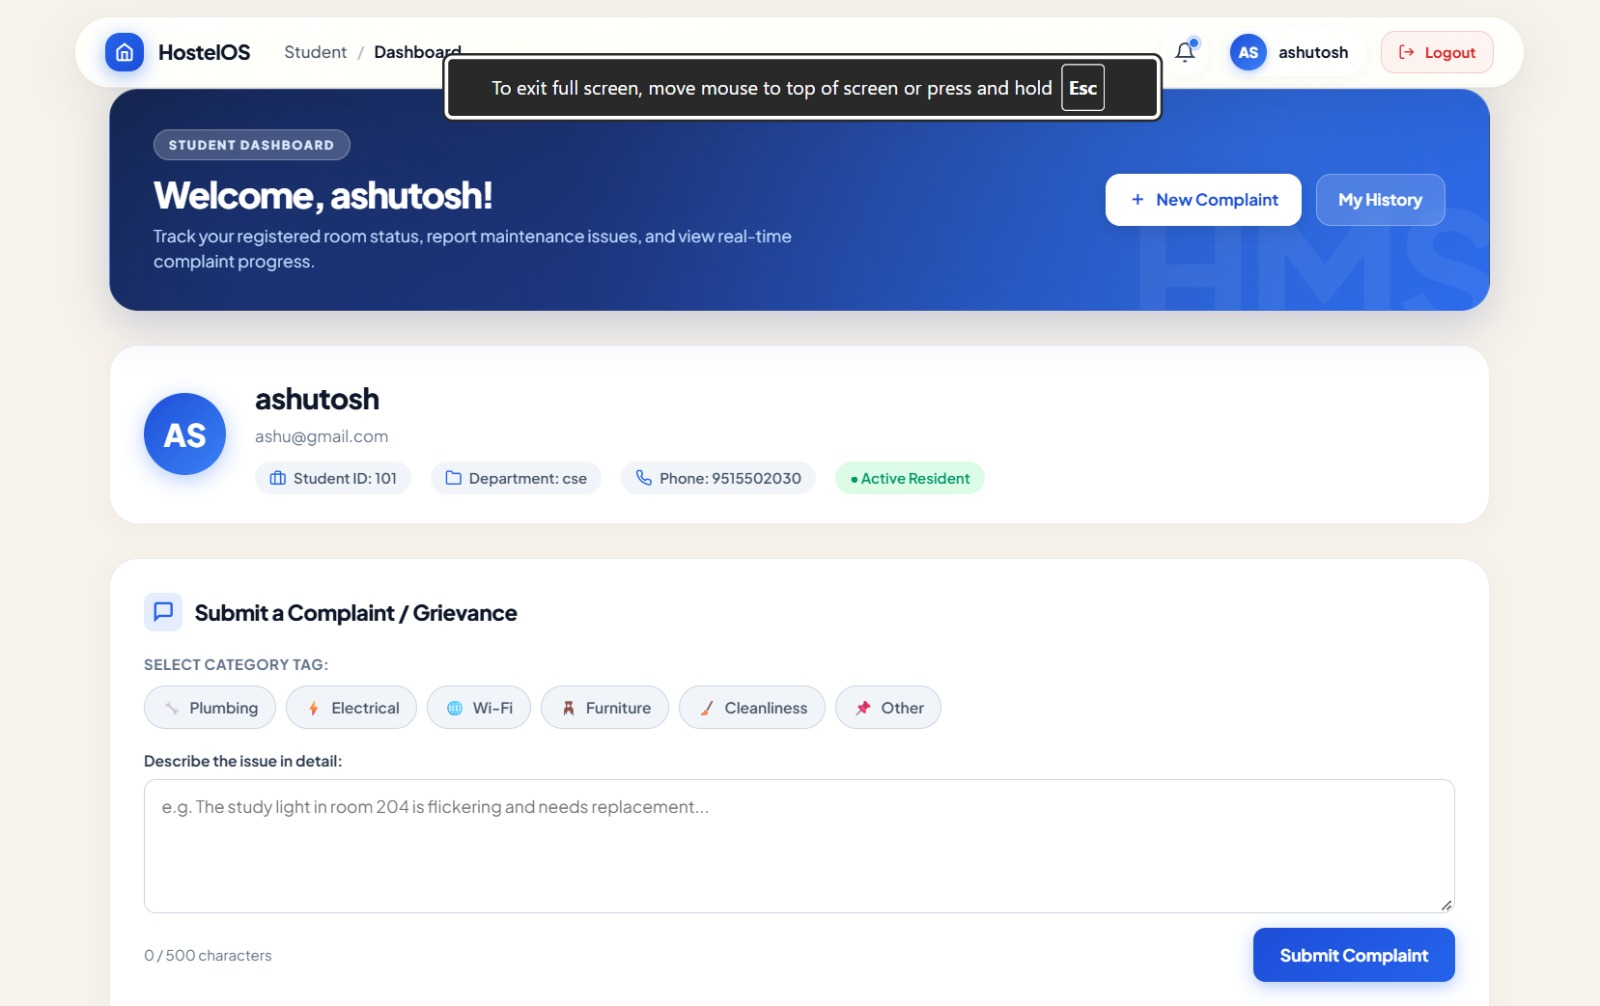
\includegraphics[width=0.95\textwidth]{student_dashboard.jpeg}
\caption{Student Resident Portal Dashboard Interface (Profile, Room Status, Complaint Form)}
\label{fig:student_ui}
\end{figure}

\subsection{Administrator / Warden Command Center Dashboard}
\label{sec:admin_screen}
Figure~\ref{fig:admin_ui} displays the Administrative Warden Command Center. This high-density operational cockpit presents real-time aggregate KPI metrics (Total Students, Total Rooms, Facility Occupancy Percentage, Available Vacancies, and Active Maintenance Complaints). Below the analytical metric cards, wardens access the room allocation matrix, student registration workflows, and grievance triage controls that allow updating complaint progression with a single click.

\begin{figure}[H]
\centering
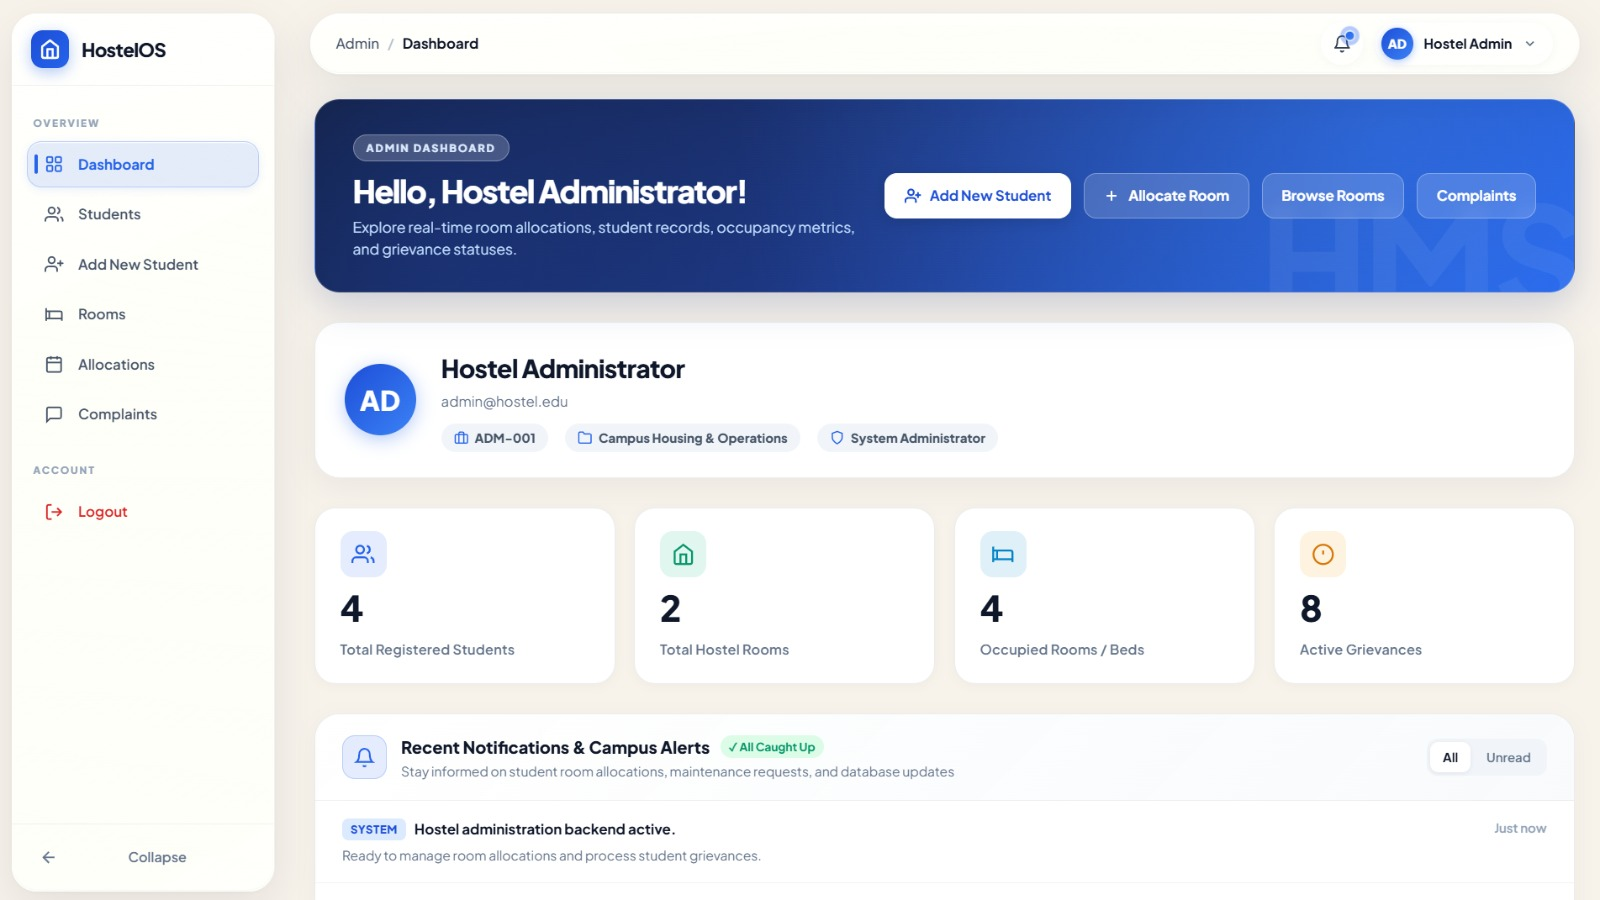
\includegraphics[width=0.95\textwidth]{admin_dashboard.jpeg}
\caption{Administrative Warden Command Center Dashboard (KPI Metrics, Room Matrix, Triage)}
\label{fig:admin_ui}
\end{figure}

% =====================================================================
% 13. Conclusion and Future Enhancements
% =====================================================================
\section{Conclusion and Future Enhancements}
\label{sec:conclusion}

\subsection{Conclusion}
\label{sec:conclusion_summary}
The \textbf{HostelOS} mini project successfully implements a robust, secure, and production-ready Hostel Management System that solves the critical inefficiencies of legacy paper ledgers and disconnected spreadsheets. By applying core Object-Oriented Programming (OOP) principles—including strict data encapsulation, domain entity modeling, separation of concerns, and dependency injection—the backend achieves modularity and high performance.

The multi-tier architecture cleanly decouples client presentation from server-side domain logic and relational persistence. The embedded C++17 RESTful application server delivers low memory overhead, sub-millisecond route response latencies, and resilient concurrency handling. The MySQL persistence tier enforces referential integrity through foreign key cascades and unique constraints, eliminating student double allocations and room overbooking. The modern web interface provides residents and hostel wardens with intuitive, responsive, and aesthetically engaging workflows.

\subsection{Future Enhancements}
\label{sec:future}
While HostelOS delivers an end-to-end management solution, several future enhancements are planned:
\begin{enumerate}
    \item \textbf{Cryptographic Token-Based Authentication (JWT):}
    Upgrading session management from identifier-based state to stateless, cryptographically signed JSON Web Tokens (JWT) with configurable expiry and refresh tokens.
    
    \item \textbf{Automated Room Allocation Optimization Engine:}
    Incorporating constraint-satisfaction and Gale-Shapley matching algorithms to pair roommates based on academic year, department, sleep schedules, and study preferences.
    
    \item \textbf{Automated Multi-Channel Notification Webhooks:}
    Integrating SMTP email services and SMS/WhatsApp gateway webhooks to notify students instantly when maintenance grievances advance to \textit{In Progress} or \textit{Resolved}.
    
    \item \textbf{Mess Billing and Hostel Fee Payment Integration:}
    Extending the relational schema with fee ledger entities, invoice generation, and secure digital payment gateway integration (UPI, credit/debit card) for hostel rent and mess subscriptions.
    
    \item \textbf{Biometric and Smart Turnstile Attendance Integration:}
    Interfacing with campus IoT hardware turnstiles and biometric fingerprint/facial recognition scanners to track student hostel entry and exit timings in real time.
\end{enumerate}

% =====================================================================
% References
% =====================================================================
\section*{References}
\label{sec:references}
\begin{thebibliography}{99}
\bibitem{cpp17} B.~Stroustrup, \emph{The C++ Programming Language}, 4th~ed.\ Addison-Wesley Professional, 2013.
\bibitem{httplib} Y.~Hirose, ``cpp-httplib: A C++11 single-file HTTP/HTTPS library,'' \url{https://github.com/yhirose/cpp-httplib}, 2024.
\bibitem{nlohmann} N.~Lohmann, ``JSON for Modern C++,'' \url{https://github.com/nlohmann/json}, 2024.
\bibitem{mysql} Oracle Corporation, \emph{MySQL 8.0 Reference Manual: C API Implementation Guide}, 2024.
\bibitem{tikz} T.~Tantau, \emph{The TikZ and PGF Packages: Manual for version 3.1.10}, \url{https://tikz.dev/}, 2023.
\end{thebibliography}

\end{document}

